\section{Method}
\label{sec:method}

\begin{figure*}[t]
\centering
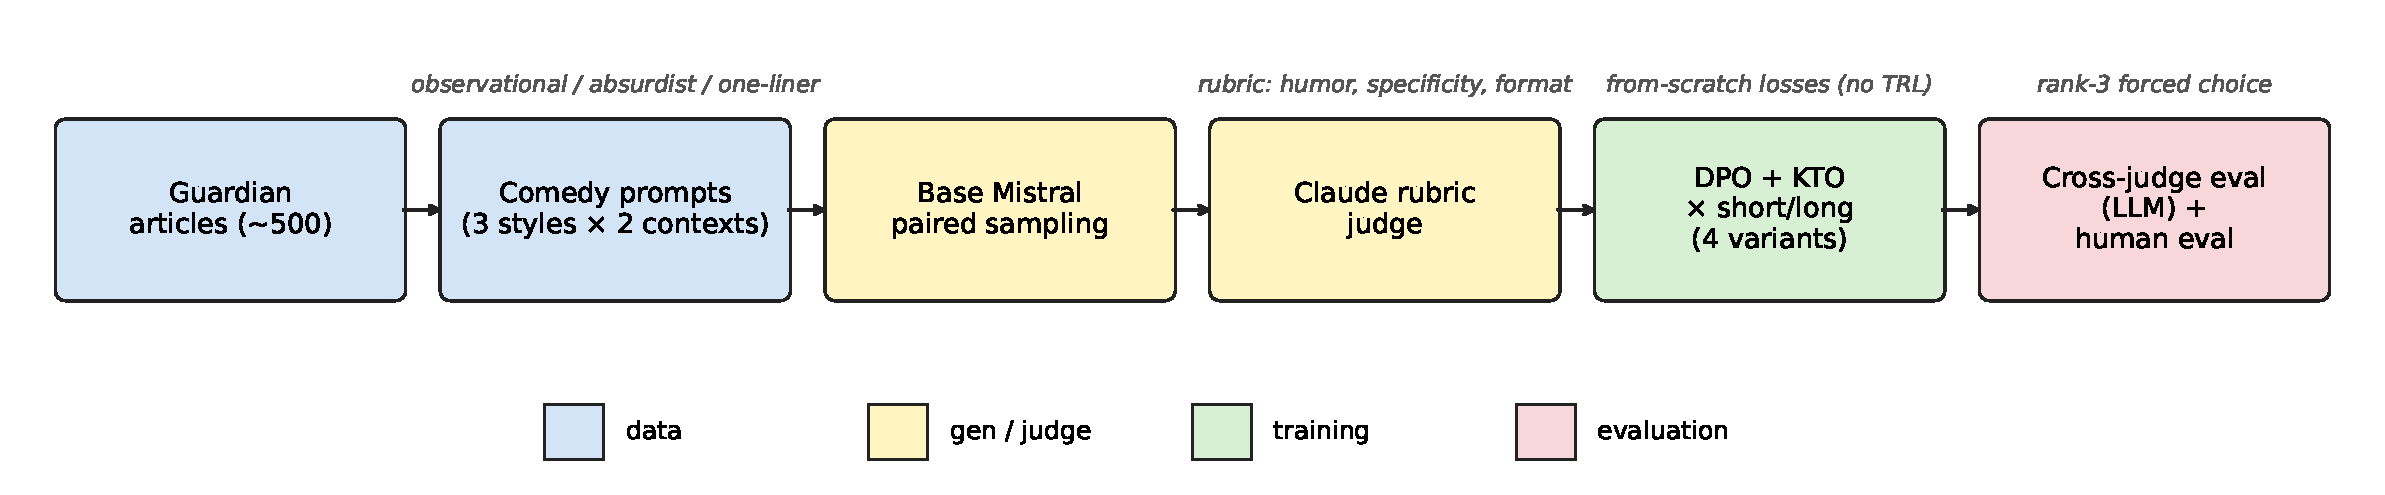
\includegraphics[width=0.98\linewidth]{figures/pipeline.pdf}
\caption{End-to-end pipeline: Guardian articles to LoRA-tuned variants to cross-judge + human evaluation.}
\label{fig:pipeline}
\end{figure*}

\subsection{Data construction}
We fetch 502 articles from the Guardian Open Platform API spanning eight sections (politics, business, technology, sport, culture, science, environment, world) and build one comedy prompt per article.  Each prompt is randomly assigned one of three styles (observational, absurdist, or one-liner), with the style label only affecting the role and task instructions; the rest of the template is identical across prompts.

\paragraph{Short vs.\ long context.}
Every prompt has two variants that differ only in their context body.  The \textbf{short} variant contains the article's headline and the first $\sim$400 tokens of the body.  The \textbf{long} variant prepends a model-generated $\sim$150-word historical backstory: we run a topic query extracted from the headline through the Guardian search API (1--18 month lookback ending two weeks before publication), retrieve the three most relevant older articles, and have Claude Sonnet 4.6 summarize them.  The role/task/output-format wording is identical across both variants, so the only experimental factor is the context body.  Figure~\ref{fig:prompt} shows the exact template with the long-only insert highlighted.

\begin{figure}[t]
\centering
\small
\setlength{\fboxsep}{4pt}
\colorbox{gray!8}{\parbox{0.92\linewidth}{\small
\texttt{<role>}You are a sharp observational comedian.\texttt{</role>}\\[2pt]
\texttt{<context>}\\
\colorbox{cyan!20}{\parbox{0.84\linewidth}{\textbf{\textit{[long only]}} \texttt{<background>}~A 150-word factual recap synthesized by Claude Sonnet 4.6 from up to three older Guardian articles retrieved via topic-query search.~\texttt{</background>}}}\\
\texttt{<latest>}~Headline + first $\sim$400 tokens of today's article body.~\texttt{</latest>}\\
\texttt{</context>}\\[2pt]
\texttt{<task>}Write a short, specific comedic take (2--3 sentences). Reference real details from the context.\texttt{</task>}\\[2pt]
\texttt{<output\_format>}Respond with only the joke. No preamble or quotation marks.\texttt{</output\_format>}
}}
\caption{Prompt template (observational style).  \colorbox{cyan!20}{Shaded region} appears only in the long variant; the rest is identical across short/long and across styles.}
\label{fig:prompt}
\end{figure}

\paragraph{From articles to preferences.}
We split 30 prompts off as the held-out evaluation set and use the remaining 472 for training/validation (10\% val).  For each training prompt we sample two candidate responses from the frozen base model at $T{=}0.9$, $p{=}0.95$ and score each with Claude Sonnet 4.6 against a fixed three-axis humor rubric: \textbf{context engagement}, \textbf{comedic technique}, and \textbf{surprise} (1--5 each, taken from a single judge call).  Let $c$ be the mean of the three sub-scores.  Two datasets are then derived from the \emph{same} scored pool:
\begin{itemize}\itemsep1pt\parsep0pt
\item \textbf{Paired preferences} (for DPO): per prompt, the higher-$c$ response is the chosen, the other is the rejected.
\item \textbf{Binary labels} (for KTO): responses with $c \geq 3.0$ are marked desirable, responses with $c \leq 2.5$ are marked undesirable, intermediate $c$ are dropped.
\end{itemize}
This co-derived sampling pool isolates the loss-function comparison from a data-pipeline confound that would arise if DPO and KTO were trained on independently-collected datasets.

\subsection{From-scratch DPO and KTO}
Implementing both losses from scratch lets us instrument internal quantities (particularly the policy-vs-reference log-probability ratio) that high-level training APIs hide, which is what makes the policy-drift diagnostic in Section~\ref{sec:experiments} possible.

\paragraph{DPO loss.} For paired data $(y_w, y_l)$ with implicit reward $r_\theta(x,y) = \log \pi_\theta(y|x) - \log \pi_\text{ref}(y|x)$,
\begin{equation}
\mathcal{L}_\text{DPO} = -\mathbb{E}\left[\log \sigma\!\left(\beta (r_\theta(x,y_w) - r_\theta(x,y_l))\right)\right].
\end{equation}

\paragraph{KTO loss.} For binary-labeled data with per-batch reference $z_\text{ref} = \operatorname{stop\_grad}(\mathbb{E}[r_\theta])$,
\begin{align}
v(x,y) &= \begin{cases} \sigma(\beta(r_\theta - z_\text{ref})) & \text{if } y \text{ desirable} \\ \sigma(\beta(z_\text{ref} - r_\theta)) & \text{if } y \text{ undesirable}\end{cases} \\[2pt]
\mathcal{L}_\text{KTO} &= \mathbb{E}\big[\lambda_y \cdot (1 - v(x,y))\big],
\end{align}
where $\lambda_\text{desirable}$ and $\lambda_\text{undesirable}$ are inverse class frequencies that rebalance the batch.  $\mathcal{L}_\text{KTO}$ is bounded in $[0, \max(\lambda_d, \lambda_u))$ regardless of how far $r_\theta$ drifts from $z_\text{ref}$; this bounded-loss property becomes important in Section~\ref{sec:ktodrift}.

\subsection{Training configuration}
Table~\ref{tab:hp} lists training hyperparameters, shared across all four variants on a single NVIDIA A100 GPU on Google Colab; only loss type and context length vary.

\begin{table}[t]
\centering
\small
\begin{tabular}{ll}
\toprule
Hyperparameter & Value \\
\midrule
Base model & Mistral-7B-Instruct-v0.2 \\
Quantization & 4-bit NF4 (QLoRA) \\
LoRA rank / $\alpha$ / dropout & 16 / 32 / 0.05 \\
LoRA target modules & q,k,v,o projections \\
Max sequence length & 1024 tokens \\
Optimizer & AdamW (paged) \\
Learning rate & $1{\times}10^{-5}$ \\
LR schedule & cosine, 10\% warmup \\
Effective batch size & 32 ($16 \times 2$ accum) \\
Max grad norm & 1.0 \\
$\beta$ (DPO and KTO) & 0.1 \\
Epochs & 10 (with early stopping) \\
Eval / save interval (steps) & 10 / 20 \\
Early-stopping patience & 5 evals \\
\bottomrule
\end{tabular}
\caption{Training hyperparameters.}
\label{tab:hp}
\end{table}

\subsection{Evaluation protocol}
For each trained variant we generate one response per held-out prompt using the \emph{best-validation-loss adapter checkpoint} for that variant (the same adapter the training loop reloads on exit after early stopping), with the base Mistral generation hyperparameters ($T{=}0.9$, $p{=}0.95$, $\text{max\_new\_tokens}{=}200$).  We evaluate every variant on the 30-prompt held-out split with two complementary signals.  The primary signal is an \textbf{LLM cross-judge}: for each prompt and each comparison (base vs DPO, base vs KTO, DPO vs KTO), the judge ranks all three generations under randomized letter labels, and we read pairwise win rates from the rank-3 ordering.  As a \textbf{secondary, human-grounded} signal, the author performed the same blinded rank-3 ranking on 30 sampled triplets (15 short + 15 long, interleaved with no context-length label); we report pairwise agreement between the two judges as a sanity check on the cross-judge.  As a fluency check we also report \textbf{perplexity} of the generated jokes under the frozen base model: it catches collapsed or off-distribution generations even when the cross-judge cannot articulate why.
